\documentclass[12pt]{article}
\usepackage{xcolor}
\usepackage[margin=1in]{geometry}
\usepackage{graphicx}
\usepackage{subcaption}
\usepackage{parskip}
\usepackage{natbib}
\usepackage{url}
\usepackage{titling}
\usepackage{sectsty}
\usepackage{float}

\allsectionsfont{\centering}
\setcounter{secnumdepth}{0}

\begin{document}

	\begin{titlingpage}
	\centering
    	{\huge\bfseries Visualizing and Predicting Influenza Cases in New York State\par}
    	\vspace{2cm}

	{\Large  A Master’s Project \\}	
	{\Large  Presented to the \\}	
    	{\scshape\LARGE Biomedical and Health Informatics Program \par}
	
	\vfill
    	{\Large  In Partial Fulfillment \\}	
	{\Large  of the Requirements for the \\}
    	{\scshape\LARGE Master of Science Degree \par}
	
	\vfill
	{\LARGE State University of New York \par}
	{\LARGE  at Oswego\par}

	\vfill
	{\Large By Daniel Truong\par}
	{\large December 5th, 2019\par}
	\end{titlingpage}


\section{Abstract}

Influenza is a contagious and potentially lethal viral disease that affects a good amount of the U.S. population every year. Preventative treatment through periodic vaccination is instrumental in mitigating the deadly effect of the disease. Other factors that could affect the efficacy of treatment include climate, geolocation, and population density. As such, for researchers to get a better grasp on the effect that the aforementioned variables play, data must be collected periodically to make assertions. This project involves visualizing the occurrences of influenza cases in New York State from 2009 to the present. Also, a couple of prediction models were tested and evaluated on data from 2018 onwards. The result was that the prediction models detected the general trend of when the cases occurred, but not the exact magnitude. A project like this is designed to be adapted for other types of diseases or different municipalities.

\newpage

\tableofcontents

\newpage

\section{Introduction}

Influenza is a viral infection that predominantly affects the respiratory system. Colloquially referred to as “the flu”, symptoms of influenza include fever above 100 degrees Fahrenheit, aching muscles, headaches, nasal congestion, and persistent coughs. In most extreme cases, influenza can lead to more serious ailments such as pneumonia, heart problems, or even death.

There are four strains of the Influenza virus: types A, B, C, and D. In a study done by  \cite{plos-one}, types A \& B are the most common infections to afflict the human body. Type C is said to be a more lethal strain, but less common compared to A \& B. Type D is a newer strain, but rarely found to affect the human body. The type A strain is the most virulent; spread vectors usually include avian species (namely aquatic birds and poultry) and human beings. From a study by \cite{virulence}, some of history’s most devastating influenza outbreaks such as the H1N1 (swine flu) and H5N1 (bird flu) strains originated from the type A strain.

One of the ways that the effects of the influenza virus can be mitigated is with periodic vaccinations (usually done as a yearly “flu shot”). The influenza vaccine is a neutralized version of the influenza virus that gets introduced into the immune system of a human being. The immune system would become provoked by the introduction of the foreign virus and generate a biological response to protect the human body. From there, if the human body were to come into contact with a strain of the influenza virus, the immune system would be trained to be able to combat the virus (and protect the human body as such). The human body must be subjected to periodic vaccines due to the ever-changing behavior of the influenza strain in such a short time.

Environmental variables can also affect the spread of the influenza virus. Amongst more populous locations, the virus can easily spread from person to person. Places like schools, office buildings, buses, and other public congregations are often common threat vectors for influenza to spread. Extra care must be given to geolocational factors if a treatment plan were to be drafted to address an influenza epidemic.

\section{Data Visualization}

A study by \cite{bmc} was done to see if the visualization of disease mechanisms helped with the “sense-making” of complex disease topics amongst the general population. What they found (albeit amongst a small sample-size population) was that the understanding of such complex mechanisms came about from the supplementing of visual representations with background information that bolstered whatever point the researchers were aiming for. In short, for researchers (investigating disease mechanisms, epidemiology, or other higher-order topics) to make their point amongst the general population, not only was it important to empirically connect their evidence to their research, but it was also imperative to visually show that connection as well.

In medicine, epidemiology is the study of factors and variables that affect population health on a locational and temporal basis. For the most part, infectious diseases are studied for their effect on population health and spread vectors. Influenza would fall into this category. To get an adequate idea of how dangerous the influenza virus can spread and find ways to combat its spread, visualizing the geographical trends of influenza infections would certainly help researchers in gaining rapid insight into its spreading trends. A study done by \cite{emerging} in Japan combined geographical evaluation with kriging analysis to not only track down the general infection cases originating in western Japan, but to also analyze seasonal trends to better target patients for preventative treatment. Another study, done by \cite{plos-ntd} in Kenya, found variances in the locational occurrences of leprosy and demonstrated a need to lock down public health policies in these areas. Having that visual association of diseases with geolocation will help researchers reach conclusions about their occurrences more coherently and rapidly.

\section{Project Methodology}

To help with visualizing and predicting influenza trends, a web-based application will be developed for this purpose. The objective of the app is as follows:

\begin{itemize}
  	\item {Display the magnitude of influenza cases in NYS per specific periods.}
  	\item {Generate a prediction model for influenza cases from 2018 to the Present.}
	\item {Use open-source technology to allow for adaptation by other municipalities.}
\end{itemize}

When developing this project, the main actors that we're concerned with developing for common users and other developers. The project defines users as professionals who will benefit from the data visualizations and predictions by viewing the generated info (i.e. NYS general population, primary care physicians, pharmacies, and other researchers primarily focused on influenza cases in NYS). Other developers are defined as users who will take the existing app and adapt it for other locations or diseases (i.e. epidemiologists, health care agencies, universities, etc.). Developing the app as a web-based program will allow access for a greater range of clients, as well as ease of use.

\section{Data Source}

NYS’ Department of Health operates a public health data repository through its Statewide Planning and Research Cooperative System (SPARCS). Researchers can get access to public use data such as (but not limited to) birth rates, locations of medical facilities, nursing home reviews, and chronic illnesses. The data that this project will be concerned with is the lab-confirmed cases of influenza (separated by county and type as far back as 2009).

When downloading the data from its source, there are a total of 59,868 records amongst 9 variables:

\begin{itemize}
	\item {\textbf{Season}: the yearly period for which the flu data was recorded}
	\item {\textbf{Region}: the geographical description of where the data was recorded (i.e. Central New York, Capital District, Western New York, Metro, etc.)}
	\item {\textbf{County}: the County of the recorded incidents}
	\item {\textbf{CDC.Week}: designation of the end-of-week (for the year) of recording }
	\item {\textbf{Week.Ending.Date}: the date that denotes the CDC end-of-week recording} 
	\item {\textbf{Disease}: whether the disease is classified as Influenza Type A, B or Unspecified} 
	\item {\textbf{Count}: the amount of lab-confirmed cases of Influenza for the specified date}
	\item {\textbf{County.Centroid}: geographic coordinates for the centroid of the county} 
	\item {\textbf{FIPS}: unique geographic code assigned to each county and state} 
\end{itemize}

Per the description of the dataset from NYS, the number of cases reported is somewhat under-represented due to the following factors: 

\begin{enumerate}
	\item The cases are only represented if an ill patient seeks medical care.
	\item A medical specimen must be collected for testing.
	\item Test results are reported to the Electronic Clinical Lab Reporting System (ECLRS).
	\item Test results come back positive. 
\end{enumerate}

As such, it can be easy to see why a breakdown of processes could contribute to an underreporting of influenza cases. In any case, the data in its present form must be cleaned up and munged further if it’s to be of use for the project. 

\section{Prediction Algorithm}

The data for the influenza cases will occur over a set period. Because we do not have any other confounding factors in the data set (that could affect flu cases), we will need to frame the prediction as a univariate analysis of time series data. This analysis will be done on a per-county basis. Two prediction algorithms will be evaluated for this purpose: ARIMA and Holt-Winters Exponential Smoothing. Because the data exhibits some seasonality (repetition over a set period), both models will be utilized for the prediction component of the project.

An ARIMA (Autoregressive integrated moving average) model is a type of regression that analyzes univariate time series data that shows some evidence of non-stationarity. An example of such a study is one by \cite{agris} where periodic cell phone signals were collected to determine trends in adoption rate by the general population. Another study by \cite{transportation} analyzes the passenger flow of inner-city expressways to predict future trends and make urban planning decisions from those trends.

Contrasting ARIMA in this project is Triple Exponential Smoothing, also known as the Holt-Winters model. Holt-Winter Exponential Smoothing is primarily concerned with forecasting future values – making predicted observations on out-of-sample observations. Holt-Winters works well if the data exhibit seasonality. One example of this model in action was a study done by \cite{usenix} at WebTV to see if aberrant behavior in network traffic could be automatically detected without needing constant human supervision. It was found that while implementing such a model could be robust, the work operations of implementing a software solution for this model were not quite optimal at the time of writing. Additionally, a study by \cite{earth} used the Holt-Winters method to forecast seasonal rainfall patterns in Malaysia. This study was used to gauge the effects of climate change on natural disaster occurrences.

\section{Data Cleaning and Preparation}

To prepare the influenza data for modeling, the different influenza types were consolidated into one influenza check. Data from the 2009 - 2018 seasons were segregated out and used as training data for the prediction model. Each county was modeled separately from the other to better evaluate possible confounding factors afterward. For each year that the data was recorded, weeks 21 through 39 (roughly mid-May through late- September) were originally omitted from the source data set. Furthermore, data from the 2014 - 2015 season was missing for numerous counties. To properly train the forecasting models, dummy data were inserted to make up for the lack of observations. All dummy observations reflect zero occurrences of any influenza cases.

The programming language R (\citeyear{rlanguage}) was used for running the prediction models, in addition to cleaning the datasets with. R package \textbf{Forecast} \citep{forecast} contains the function \textit{auto.arima()} that will be used for training the forecasting algorithm. Meanwhile, the base R package has the \textit{HoltWinters()} function that will be used for the exponential smoothing prediction. The data from the 2018-2019 and 2019-2020 season were used to test the efficacy of the prediction algorithms. In all, after cleaning the data, there were 29,078 observations in the training set and 3,720 observations in the test set.

\section{Software Implementation}

To prepare the dataset for use with the interactive data map, R Studio was used to import the cleaned dataset from SPARCS. R Studio leverages the R programming language to allow researchers and developers to run statistics and transformations on datasets in a rapid manner.

The \textbf{Shiny} package \citep{shiny} for R was used to construct the user interface for the interactive data map. Shiny leverages datasets (loaded in R Studio) to create HTML5-based applications for clients to interact with. Shiny will allow us to display a map of NYS and plot circles to represent the magnitude of illnesses for each county. The map component leverages the \textbf{Leaflet} package \citep{leaflet} to render the map. The completed app can then be uploaded online to ShinyApps.io or hosted on a dedicated web server. 

\section{Finished Product}

The app has three components to it: a \underline{map} view, a \underline{data table}, and a section with \underline{predictions} for the 2018-Present flu season. The map view (Figure \ref{fig:flu-cases}) shows a map of NYS with small red dots over each county. The radius of the dots is proportional to the number of flu cases reported per season and week (both variables are user-controllable via a dropdown box towards the side). The larger the dot, the more flu cases were reported for that county. If a user selects a date within the 2018-2019 season range, they will also see blue and green colored dots of varying sizes. The blue dots represent the predicted amount of flu cases from the ARIMA model and the green dots represent values predicted from the Holt-Winters model. 

\begin{figure}[H]
\centering
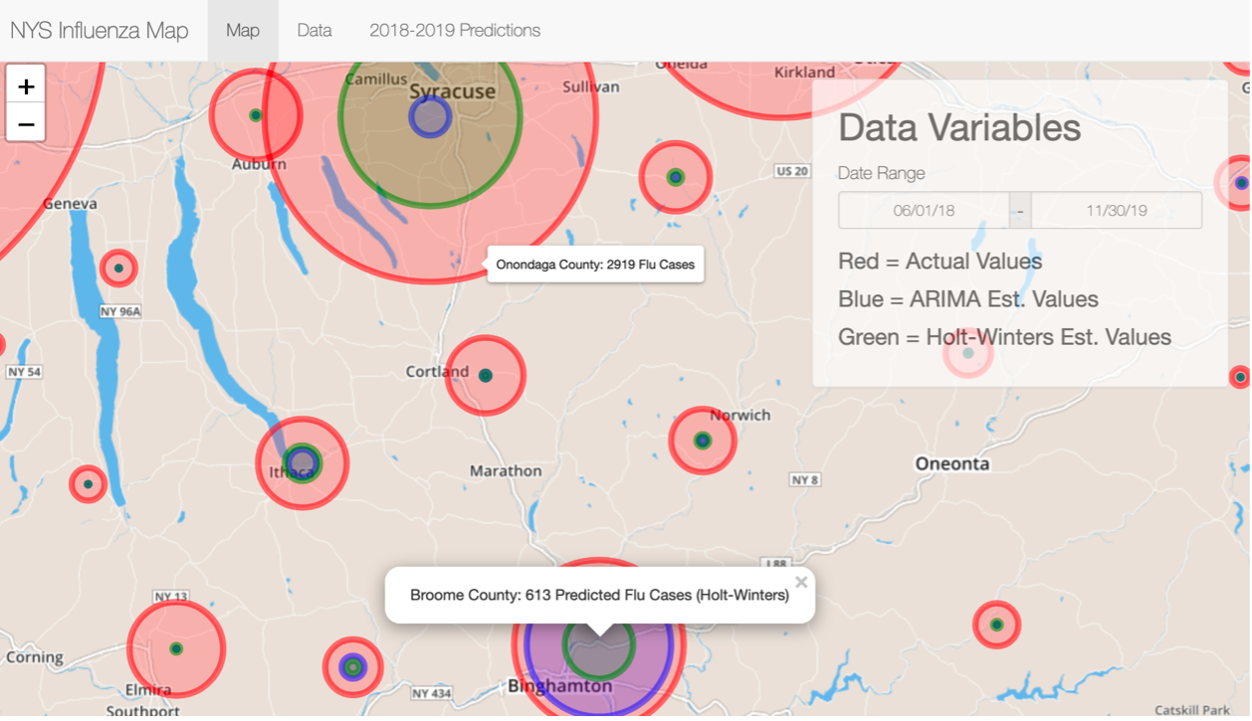
\includegraphics{Picture1.png}
\caption{Map View showing flu cases (actual and predicted) in the Southern Tier.}
\label{fig:flu-cases}
\end{figure}

\begin{figure}[H]
\centering
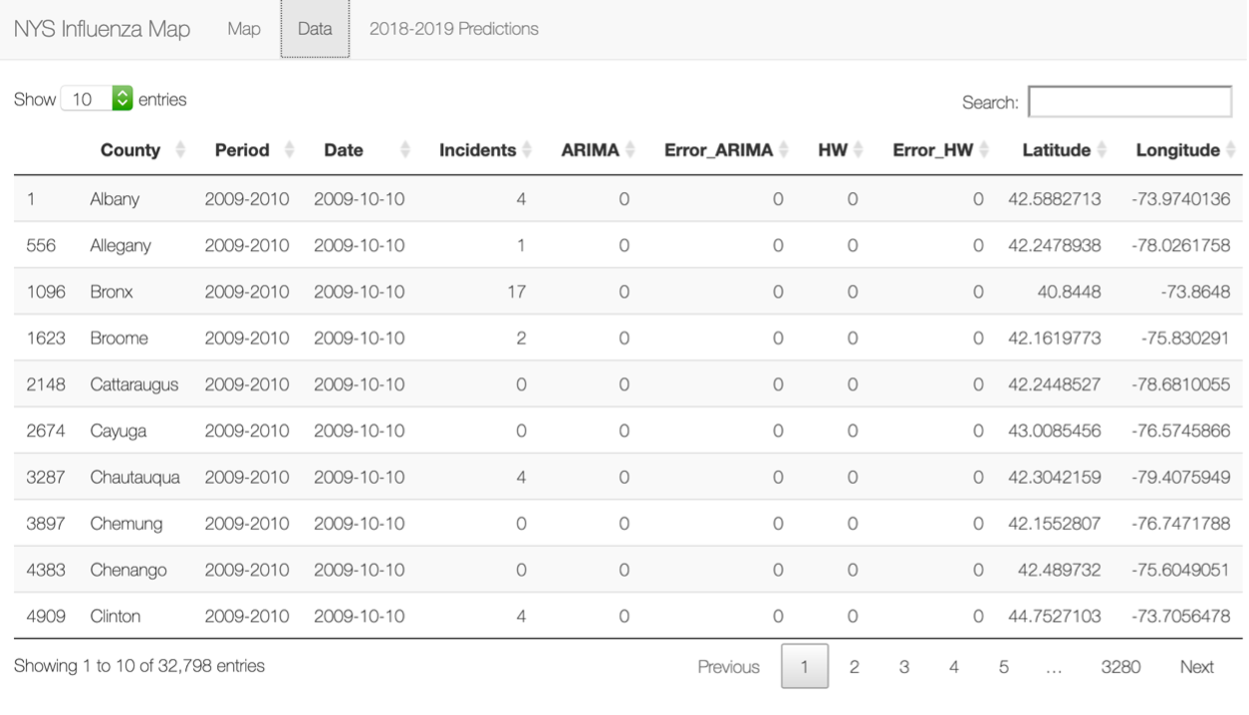
\includegraphics{Picture2.png}
\caption{Data Table}
\label{fig:data-table}
\end{figure}

The data table (Figure \ref{fig:data-table}) shows the cleaned-up data set for the user to explore. One can use the embedded search function to look for specific data on a county level, year, or season. Lastly, the prediction component (Figure \ref{fig:prediction}) shows a time-series plot of actual observed flu cases vs. what the prediction algorithms have analyzed. The solid line represents the actual observations while the dashed and dotted lines represent the predicted observations (the ARIMA and Holt-Winters models respectively). The MSE (Mean squared error) for the forecasting model is also shown.

\begin{figure}[H]
\centering
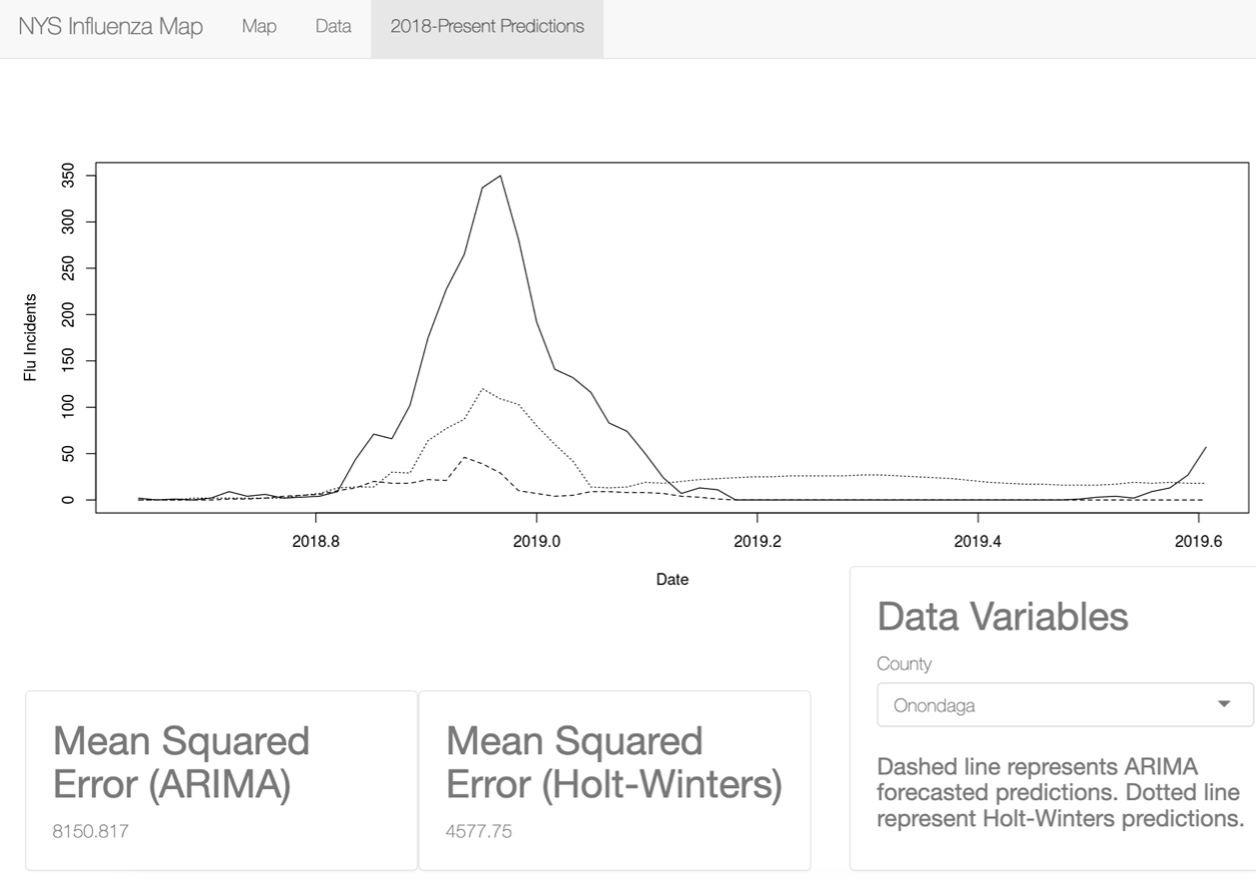
\includegraphics{Picture3.png}
\caption{App prediction component}
\label{fig:prediction}
\end{figure}

\section{Evaluation}

When it comes to evaluating the accuracy of the prediction models in each county, we find mixed results. If we evaluate using MSE (see Figure \ref{fig:mse} below), we find that some models work well for certain counties over one another.

\begin{figure}[H]
\centering
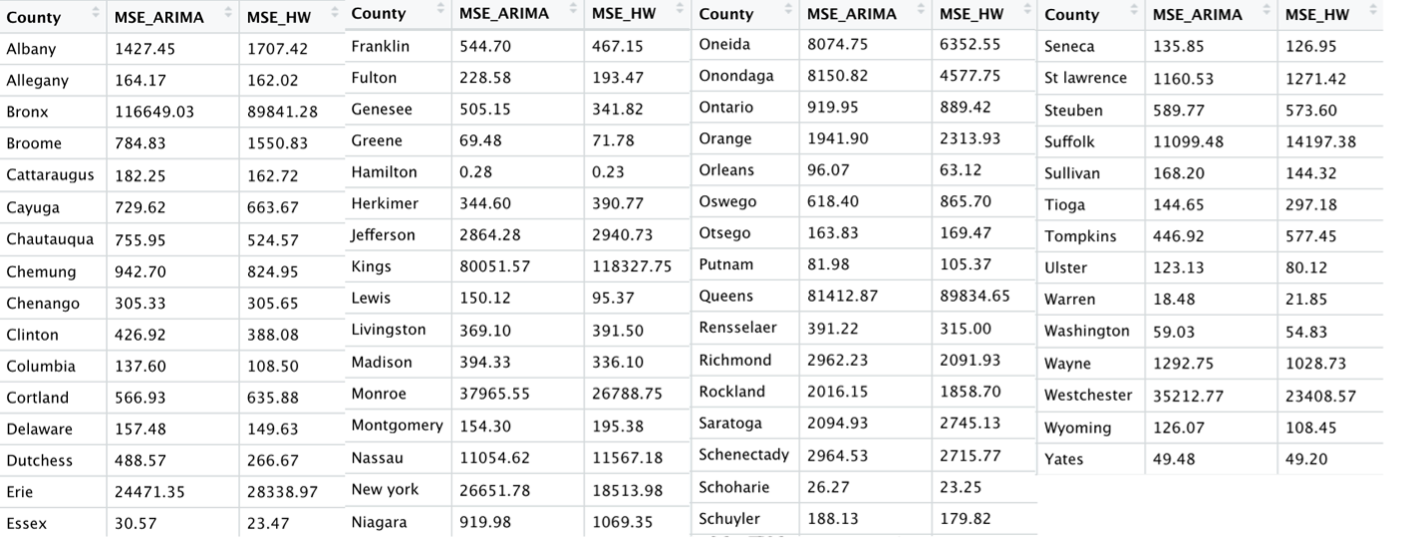
\includegraphics{Picture4.png}
\caption{Table of MSE values}
\label{fig:mse}
\end{figure}

Visually interpreting the results, we find that the predicted results generally reflect the temporal trends for when influenza occurs, but not the exact magnitude of the cases. Figures \ref{fig:broome} and \ref{fig:nassau} show this in effect.

\begin{figure}[H]
\centering
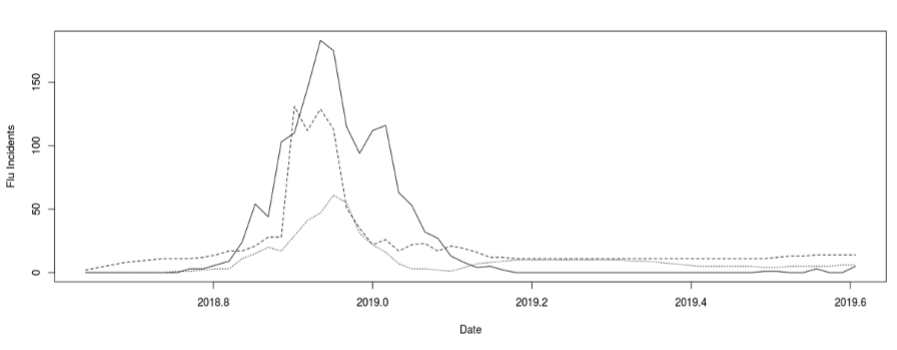
\includegraphics{Picture5.png}
\caption{Predicted vs. Actual flu cases for 2018-Present for Broome County. Dashed lines represent the predicted cases.}\label{fig:broome}
\end{figure}

\begin{figure}[H]
\centering
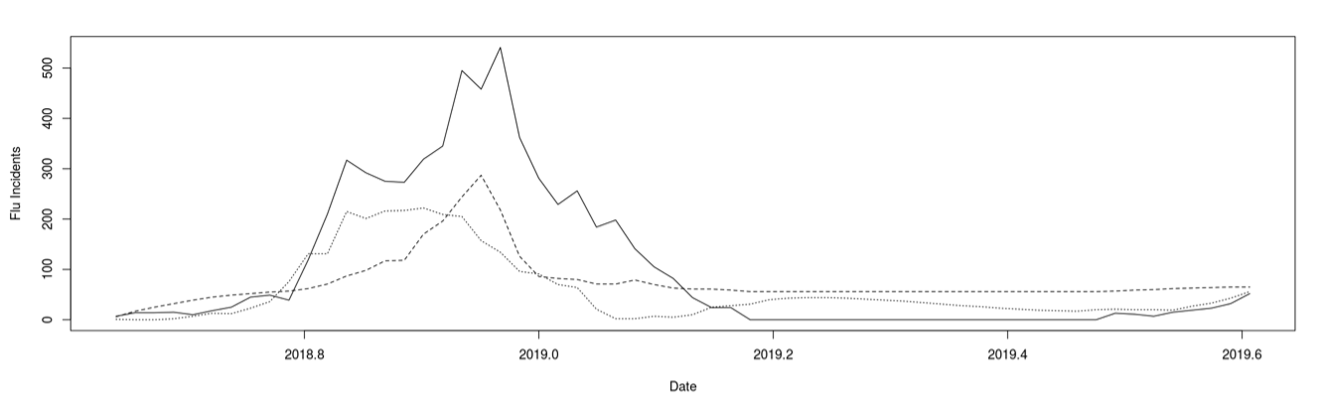
\includegraphics{Picture6.png}
\caption{Predicted vs. Actual flu cases for 2018-Present for Nassau County.}\label{fig:nassau}
\end{figure}
 
\section{Conclusion}

The prediction models as-is tend to match well for seasonal trends in influenza data, but not for the volume of cases. This could be due to factors such as missing data affecting the models, population changes, socioeconomic demographics, or confounding factors (i.e. H1N1 influenza strain of 2009). If this app is to be adopted for widespread usage amongst researchers, additional prediction algorithms will need to be further explored; ideas to refine this component could entail gaining additional data from the U.S. Center for Disease Control or exploring the prediction as a function of a multivariate linear model. The user interface will also need additional work to be optimized on mobile interfaces; the spirit of this software package is to be running on a 7 or 10-inch mobile tablet for quick and easy evaluation amongst medical professionals. As it stands, the app is primarily optimized and tested on a desktop environment. If this app is to be utilized quickly and efficiently by fellow researchers, further testing on mobile environments will be necessary to ensure that the app meets ADA Standards for Accessible Design.

\newpage
\nocite{*}
\bibliographystyle{apalike}
\bibliography{apa-references}


\end{document}